\section{Approach}\label{sec:approach}
The goal of our research is to create a system that allows gesture-based communication between the user and smart devices.
We feel that allowing users to point and control devices will give the best interface. 
This approach requires accurate indoor location, a wearable that can recognize gestures and a hub for interoperability between the wearable and the smart devices. 

\subsection{Indoor Location}
In order to determine which device the user points at and thereby intends to control, 
it is necessary to determine the locations of the devices in the system relative to the user.

The focus of this project is not to position devices and as such it was not the intention to spend time developing an entire solution for positioning devices indoors. 
Instead it was desired to find an existing product that could be used to facilitate indoor positioning.
The solution should be available in the early phases of the project in order to start building the system based on the solution for positioning.

Ideally users of this project should be able to control any device that fits within the concept of Internet of Things he owns, 
the price for any device needed to position each controllable device should be low. 
If a user owns several devices that can be controlled using gestures and an extra device is needed for each in order to preform the positioning, 
the price of such a device should be at a minimum.

It is assumed that users already own one or more devices that fit within the concept of Internet of Things and possibly are early adapters of such technology, 
it is assumed they have some technological expertise. 
However, it easy to imagine that this project can be used in an office environment where employees of varying technological expertise work or in health care. 
Therefore users may have a varying degree of technological expertise and it should be easy to extend the solution with new controllable devices.

Naturally the accuracy of the solution used for indoor positioning plays an important part. 
\Cref{fig:indoor-positioning:incorrect} shows the consequence of an incorrect location. 
If a lamp is estimated to be at another location that it is actually located, 
the user must point to an incorrect location in order to control the lamp.
Furthermore if the estimate is too wide, that is, the given area in which the lamp is located is very big, 
there is a greater risk that locations overlap. 
Overlapping locations causes a complexity as it is necessary to determine which device the user desires to control if he points at the overlap as visualized in figure \ref{fig:indoor-positioning:overlap}.

\begin{figure}[!htb]
    \centering
    \begin{minipage}[t]{0.45\textwidth}
        \centering
        
\includegraphics[width=0.6\textwidth]{images/incorrect-positioning-estimate.png}
        \caption{Incorrect location estimate. The estimate is visualized as a striped circle.}
        \label{fig:indoor-positioning:incorrect}
    \end{minipage}\qquad
    \begin{minipage}[t]{0.45\textwidth}
        \centering
        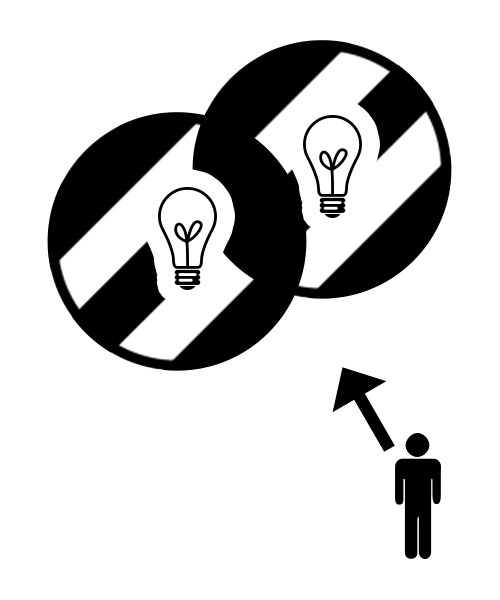
\includegraphics[width=0.6\textwidth]{images/positioning-overlap.png}
        \caption{Overlap of estimated positions. The estimates are visualized as a striped circle.}
        \label{fig:indoor-positioning:overlap}
    \end{minipage}
\end{figure}

Based on the above the following criteria for assessing potential solutions can be outlined.

\begin{itemize}
    \item Availability
    \item Price
    \item Ease of use
    \item Accuracy
\end{itemize}